\chapter{Ontologies} \label{ch:ontologies}

\todo{This is an easy story to tell if you walk through the
slides from your last committee meeting, and then answer any remaining
questions below.}

A formal system for describing scientific workflows would be valuable for a
variety of reasons. Perhaps most importantly, this includes being able to
determine what types of systems need to be implemented to successfully execute
the workflow. This is fundamentally a question about our ability to model our
workflows thoroughly without building out a fully functional system, which is
common at present. It is not clear that this model will continue to scale up
efficiently as workflows become more distributed, hierarchical, and mixed
because of the associated increase in complexity. 

One important tool in understanding complex computing systems is an ontology.
An ontology captures knowledge about a system in a formal way. This includes
capturing details about entities, classes of entities, entity properties, and
the relationships between these things. Ontologies are usually recorded in a
graph data structure. The graph can be modified, linked, or merged with other
ontology graphs to create an even greater understanding of a topic.

This chapter introduces ontologies with a focus on how they can be used to
better understand different types of workflows, workflow management systems,
and workflow data models. First, common properties of ontologies are reviewed to
provide a basic understanding of their use. Second, a short example is provided
to illustrate their use in encoding real-world data. This includes an
illustration of why ontologies are sometimes favored over taxonomies. Finally, a
common set of tools for working with ontologies is presented to illustrate how
ontologies are created in formal ways that are machine-readable, ready for
distribution, and use in larger applications.

*Why do ontologies matter here?

*Ontology versus taxonomy

*How can this be written in plain text, without invoking RDF?

*What does this look like in RDF?

*What is RDF?

*What is the semantic web?

*How does this jive with scientific workflows?

\section{Features of Ontologies}

Ontologies are commonly described using special ontology languages, such as the
Web Ontology Language (OWL), or modeling languages like the Unified Modeling
Language (UML). There are a number of common features found across these
languages, some of which are useful for the following discussions. 

\subsection{Properties}

Entities in an ontology can have properties that describe their makeup. Some
entities, such as primitive double precision floating point numbers have their
value as their only property. However other entities, such as a computer, may
have many properties including hardware peripherals and non-physical properties
including cost. Entities are connected to properties through relationships.

\subsection{Objects and Classes}

An object is a specific entity that has been initialized with some default.
A simple equation $x = 5$ could be used to denote that the object $x$ has the
value five. A set of objects is defined by a class. Objects may sometimes be
called instances or individuals, and all three terms are used interchangeably
herein.

Classes define the properties (or in some definitions links to properties) and
required relationships for objects. One special relationship is the
\textit{Inheritance} relationship. This relationship indicates that one class
must have - inherit - the properties and relationships of another class, called
its ``parent.'' Classes that inherit from other classes are said to be
subclasses of their parent ``base'' class.

A trivial example would be a class Money with subclasses Coin and Bill. In
United States Currency, Coin would have subclasses Nickel and Penny. A roll of
pennies from a bank would contain fifty pennies, all of which would be objects
or insances of the Penny base class.

\subsection{Ontological Openess}

Ontological openess is the quality of a graph to be left open to modification.
Open ontologies are capable of describing knowledge from multiple perspectives
that more accurately describe the nature of the object. It is possible for
individual entities within the ontology to be modified, or for new graphs to be
linked to the existing graph to provide these different perspectives.

Consider, for example, a tea cup. What is it? Is it a vessel for holding tea or
is it clay? Is it plastic? Is it red, blue, or covered with a picture of
Captain Picard? Was it a gift? Is it warm to the touch? Is it also possible to
hold other liquids? By leaving an ontology that only describes what the tea cup
can hold open to extension, all of these properties can be linked to describe a
clay tea cup that can also hold coffee, that has a picture of Captain Picard on
it, that was a gift, and which was warm when the author started writing this
page.

\section{Case Study: A professor, a businessman, and a pilot}

It is straightforward to create a complex example that is still relatively
simple enough to be educationally valuable. Consider six simple statements about
a thesis committee:

\begin{itemize}
\item Mike, Mike Jr., and Jack are full professors.
\item John T. and Arjun are adjunct professors.
\item John D. is a research professor.
\item Mike is also a businessman and a pilot.
\item Mike Jr. is Mike's son.
\item Mike and John both play guitar.
\end{itemize}

\begin{figure}[htbp]
\centering

\includegraphics[width=\textwidth]{figures/tc-tax-v2.png}
\caption{Common data structures and their relationships in ICE.}
\label{data-arch}
\end{figure}

\begin{figure}[htbp]
\centering
\includegraphics[width=\textwidth]{figures/tc-tax-v4-wErrors.png}
\caption{Common data structures and their relationships in ICE.}
\label{data-arch}
\end{figure}

\begin{figure}[htbp]
\centering

\includegraphics[width=\textwidth]{figures/tc-ont-classes.png}
\caption{Common data structures and their relationships in ICE.}
\label{data-arch}
\end{figure}

\begin{figure}[htbp]
\centering
\includegraphics[width=\textwidth]{figures/tc-ont-instances.png}
\caption{Common data structures and their relationships in ICE.}
\label{data-arch}
\end{figure}


\section{The Resource Description Framework}

*What is RDF?

\subsection{RDF Schema (RDFS)}

\subsection{Web Ontology Language (OWL)}

\subsection{Our case study in RDF}

\section{A Workflow Ontology}

A workflow may be defined as a collection of tasks that are executed in some order by human and non-human actors. A workflow problem can then be defined as any problem that is solved the the execution of a specific workflow. Many systems exist that can execute workflows encoded in one or more \textit{description formats} for both business and scientific problems. There are predominantly three types of scientific workflows: High-throughput \cite{}, Modeling and Simulation \cite{}, and Analysis \cite{}.

Workflow problems of any of type can be decomposed into three required components: The workflow description, the \textit{workflow engine} that executes the workflow based on the description, and the data required to fully describe and execute the workflow. The latter may include - but does not necessarily require - metadata that describes the contents of the data itself, bulk data including values and quantities of interest used in the workflow. (For the purposes of this work, it is sufficient to consider provenance information as a type of metadata.)